\chapter{Software Requirements \& Survey}
\label{ch:software_requirements}

In order to assess which technologies to use for a new project, one first has to take into account the kind of software product to build, the sector of the economy it will be used in as well as the specifics and constraints of the environment it's going to operate and interconnect in. Let us first take a closer look at those points:

\begin{itemize}
	\item \textbf{The kind of product} to construct will often determine some core technologies: Building a messenger app requires real-time behavior some statistical product suite would never make use of. Likewise, an autonomous control system of a space probe will also depend on time-critical components, but in a different way than a messenger app, relying strongly on a constant rate of throughput, whereas a message flow will not be critically disturbed by a lag or latency disruption every now and then.
	\item \textbf{The industry sector} largely determines requirements in the form of compliance or industry certification. For instance, whereas the security concerns in a normal end-user centered application might be dealt with with relatively moderate levels of effort, applications employed in the financial or even medical sectors will in all probability have to satisfy additional security demands such as audit trail systems or compliance to specific data formats and standards.
	\item \textbf{The technical environment} a system is operated in will influence its shape and behavior as well. A relatively disconnected and isolated system like a statistical module (which e.g. outputs some results on a nightly basis) will be modeled differently than a web-based, cloud-oriented service incorporating many interfaces and API calls to dependent background or partner services.
\end{itemize}

In the following sections, we are not considering the entire SW development workflow from an economic / managerial point of view, but just the technological aspects of it. Let us first realize the differences between software development today and the way it was usually conducted as short as only 2 decades ago.

The traditional software development process as followed throughout the first decades of the existence of our field has been relatively simple: upon setting a goal for functionality or any other measurable entity (code module, UI section), a continuous iterative process of writing some lines of code, re-compiling, testing (automated or manual) and bug fixing was all, or most, that was necessary to arrive at some usable product. Modern applications, however, especially web-based ones (and that includes all kinds of mobile apps that have seen their rise over last decade) operate on many different moving parts:

\begin{itemize}
	\item Some server-side backend which coordinates incoming requests and provides consistency across business logic and database layers. This is probably the part with the greatest similarity to traditional, client-only or centralized software (development). I would also include old-fashioned web 'applications' (and certainly websites) in this environment, as a browser-based GUI alone without much processing or business logic going on, does not really fall into the category of a distributed application.
	\item A client part in the form of a modern in-browser based app (like GMail, Google Docs or Office365) or any mobile app executing on a contemporary mobile device.
	\item Some background-services, mostly in separated modules distributed over one or many servers worldwide, including interfaces to dependent services, isolated REST services (like a search portal for medical professionals inside a larger healthcare application) or microservices: sub-components of the business logic implemented directly on a database level, as implemented in the Foxx application micro-framework inside the multi-model database ArangoDB \citep{Foxx2014}.
	\item Where needed, a visualization module will have to be provided which resides on the client side but is logically separated from the 'normal' business and communication logic of that module. In browsers, this can either be written in normal DOM code, SVG, Canvas, or WebGL (we don't want to mention earlier technologies that are fortunately falling from grace rapidly...).
\end{itemize}

In addition to this generic complexity, we have to deal with a different workflow cycle even on the level of individual developers: Whereas 15 years ago somebody could set up some HTML files, include some JavaScript files, iteratively add new snippets of code and check the results by reloading the browser, even this small part of the development cycle has changed dramatically over the past 10 years - new Meta-languages like Typescript or Coffeescript on the language side, HTML-meta-markups like HAML, CSS preprocessors like Sass/Scss/Less as well as the integration of modern testing libraries makes a simple browser reload a technique of the past.

Those new methods provide great opportunities (but also challenges) even for the single programmer, which require a whole execution and deployment infrastructure, as depicted in Figure~\ref{fig:webdev_cycle_components} and described in the following sections.

\begin{landscape}
\begin{figure}[ht]
	\centering
	\hspace*{-1cm}
	\vspace*{1cm}
	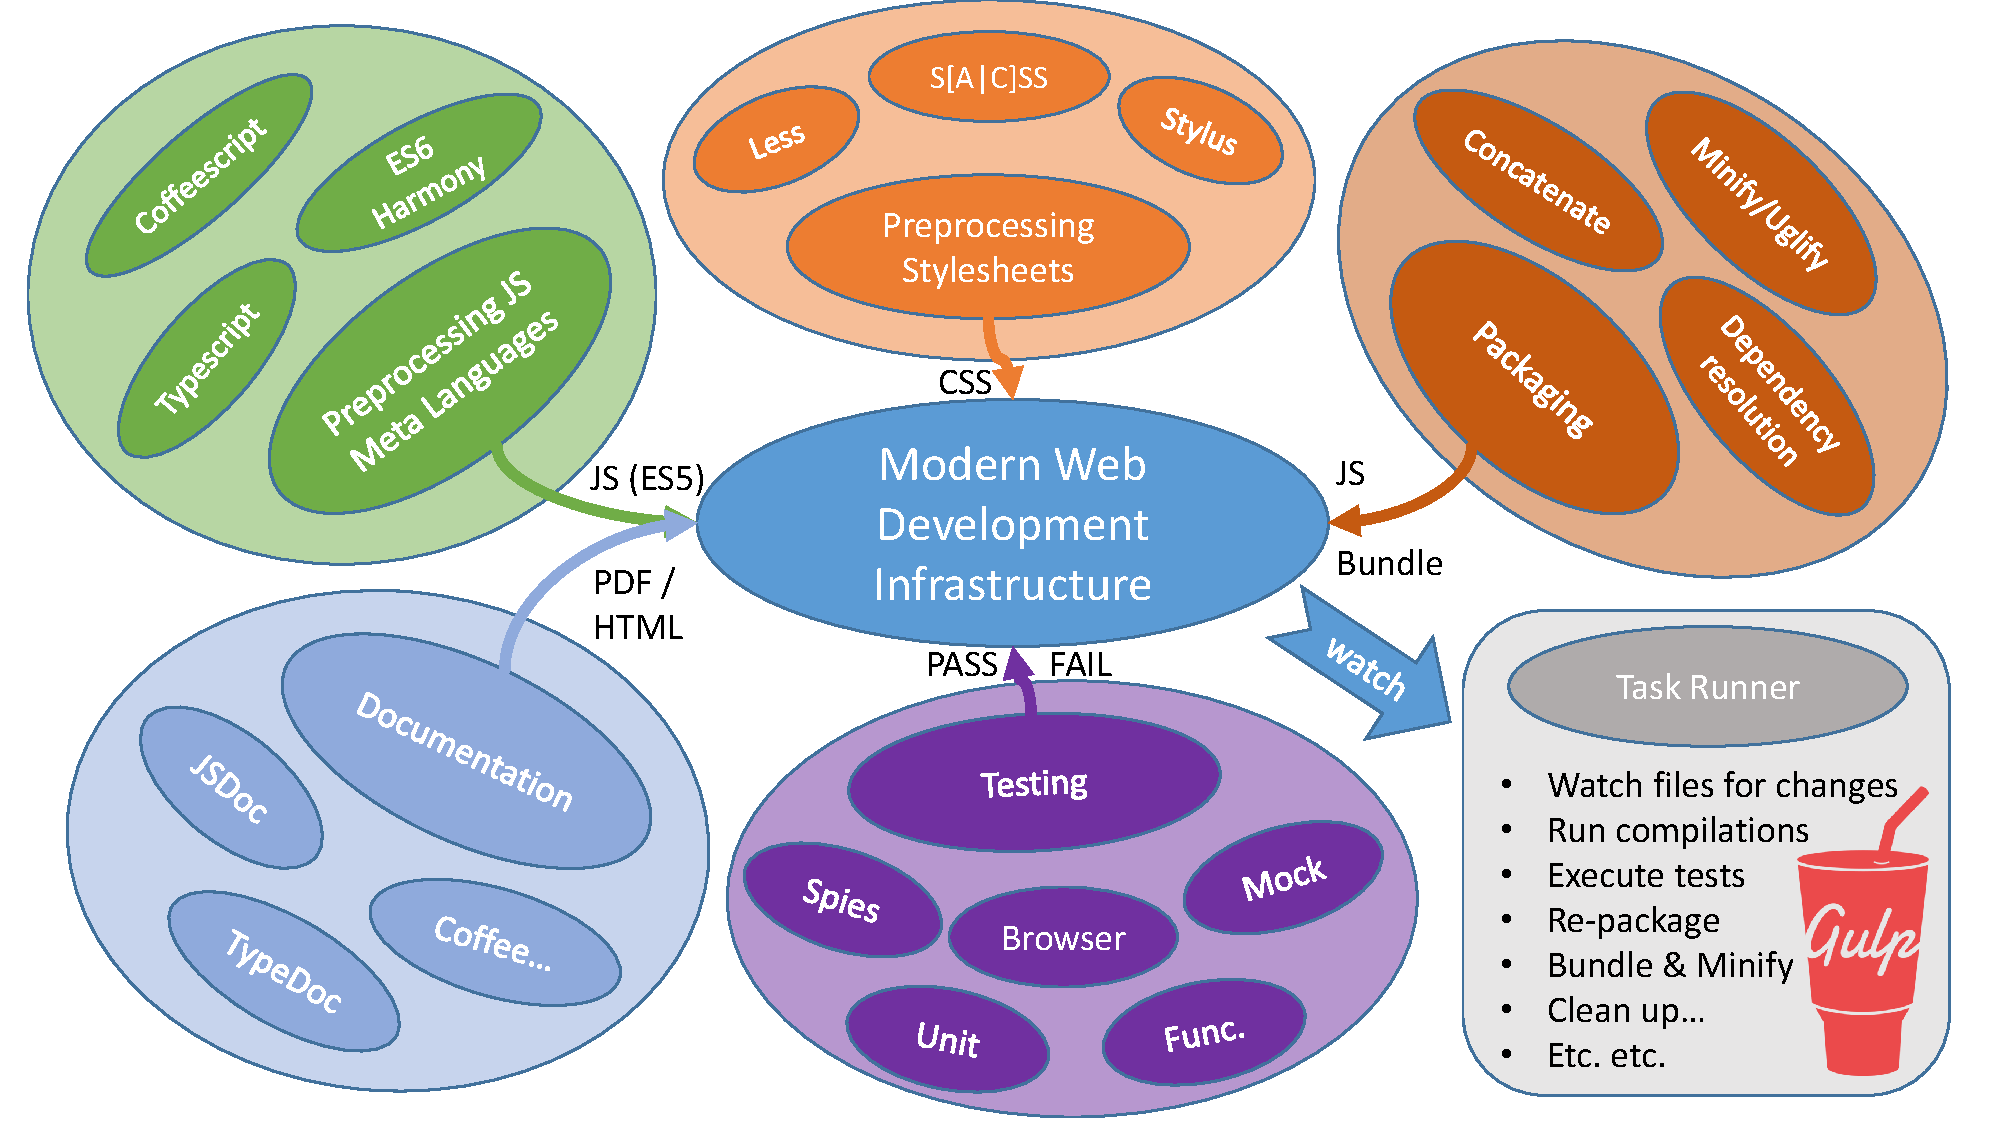
\includegraphics[width=1.8\textwidth]{figures/Modern_Web_Dev}
	\caption{Modern Web Development Component Diagram}
	\label{fig:webdev_cycle_components}
\end{figure}
\end{landscape}


\section{Graphinius JS}
\label{library}

	The components presented in this section correspond with the graphical elements in Figure~\ref{fig:webdev_cycle_components}.

	\subsection{Preprocessing (compiling) JS Meta Languages}
	\label{ssect:language}
	
		\subsubsection{Javascript / ES6}
		\label{sssect:js_es6}
		
		Although the JavaScript language was put together by Brendan Eich of the Netscape company within 3 weeks in 1994 (when it was initially called LiveScript, and in 1995 renamed to JavaScript in a marketing attempt to jump on the Java-hype bandwagon), it turned out to be a nifty little language for general in-browser development and computations. JavaScript is a prototype based language, which means that it uses pointers to parent objects instead of class instantiations, features first-order functions (functions which can generate functions) and function-as-object passing, which is ideal for callback-based implementations of the visitor pattern, even more so as JS functions are automatically closures (functions or lambdas that have, regardless of their execution context, full access to their original definition scope).
		
		After almost two decades however, the JS development community felt that requirements on modern web-based product had increased so drastically, that traditional JavaScript could only partially serve them anymore. Problems are - amongst others: 1) the lack of an explicit type system (which is crucial for larger software projects), 2) the lack of an implicit module system allowing for requiring other files or packages (except in the form of browser script tags), 3) the lack of a chaining system for async callbacks (which resulted in the notorious 'pyramid of doom'), 4) the somewhat peculiar functional scoping, which is mostly an entrance barrier to developers of other languages, as well as 5) a general lack of elegant language constructs (like deconstruction of objects into variables etc.).
		
		While some of those problems have been addressed even in the context of ECMAScript 5 (like the introduction of promises to replace nested callback functions), many shortcomings could only be addressed by external libraries, which polluted the workflow with additional dependencies not needed in more sophisticated languages and often increasing the JS download size by hundreds of kilobytes, which can become a problem on mobile devices.
		
		ECMAScript 6 (codename harmony) is an overhaul of the JavaScript language featuring classes, a new keyword for the familiar block scoping ('let'), as well as an integrated module system allowing to require external files even inside the browser. The greatest obstacle to using ES6 today is the lack of complete support across all browser vendors - this is where ES6-to-ES5 compilers like \textit{Traceur} or the more popular \textit{Babel} come in. As far as syntax goes, ES 6 cleans up some keyword usages in order to make code more readable (samples taken from \url{http://es6-features.org/}):
		
		
		\begin{lstlisting}[caption={ECMAScript 5 (usually referred to as 'JavaScript') version of functional programming using the natively built-in mapping function.}, label={fig:ECMAScript5_mapping}, language=JavaScript]
	odds  = evens.map(function (v) { return v + 1; });
	pairs = evens.map(function (v) { return { even: v, odd: v + 1 }; });
	nums  = evens.map(function (v, i) { return v + i; });
		\end{lstlisting}
		
		
		\begin{lstlisting}[caption={ECMAScript 6 equivalent to the above code.}, label={fig:ECMAScript6_mapping}, language=JavaScript]
	odds  = evens.map(v => v + 1)
	pairs = evens.map(v => ({ even: v, odd: v + 1 }))
	nums  = evens.map((v, i) => v + i)
		\end{lstlisting}
		
		Although ES6 is a great improvement over ES5 in many respects, it still lacks an explicit type system and interfaces (which can guide an IDE in it's analysis regarding Code Completion and IntelliSense). It was therefore not considered the best option for the development of a potentially large library as GraphiniusJS.			
		
		\subsubsection{Coffeescript (CS)}
		\label{sssect:coffeescript}
		
		Coffeescript was an attempt to make JavaScript code more readable as well as writable. It was apparently inspired by the clean syntax used in modern scripting languages like Ruby or Python and adopted the use of whitespace as control characters like Python (but not Ruby). Most of the language was based on using 'syntactic sugar' to abbreviate otherwise verbose JS code. For instance, the  \textit{this} variable was replaced by the  \textit{@} sign, the return statement at the end of a function became superfluous, and the lambda operator \textit{->} was introduced as a shortcut for the \textit{function} keyword in normal JS. Examples taken from \url{http://ricardo.cc/2011/06/02/10-CoffeeScript-One-Liners-to-Impress-Your-Friends.html}
		
		\begin{lstlisting}[caption={Two versions of the same mapping functionality in CoffeeScript}, label={fig:Coffeescript_mapping}, language=JavaScript]
	[1..10].map (i) -> i*2
	i * 2 for i in [1..10]
		\end{lstlisting}
		
		Like ES6, Coffeescript is compiled down to ES5 through it's own coffee compiler. As much as the idea of CS is neat and very justified for individual developers, the use of whitespace as control characters can add some additional hassles if working in a team; only slight deviations in the individual setup can cause serious problems, like the use of editors that use different representations for tabs (tab vs 2 spaces vs 4 spaces) or different line ending symbols (Windows vs. Mac vs. Linux). Furthermore, CS did not resolve the lack of an internal module system or the lack of an explicit type system, and was therefore not considered for Graphinius JS.
		
		
		\subsubsection{Typescript}
		\label{sssect:typescript}
		
		
		
		
	\subsection{Testing}
	\label{ssect:testing}
	
		\subsubsection{Jasmine}
		\label{sssect:jasmine}
		
		\subsubsection{Mocha / Chai(!)}
		\label{sssect:mocha_chai}
		
		\subsubsection{Mocking Library (Sinon)}
		\label{sssect:mocking}

		\subsubsection{Selenium(??)}
		\label{sssect:selenium}
		
	
	\subsection{Documentation}
		\label{ssect:documentation}
		
		\subsubsection{JSDoc}
		\label{sssect:jsdoc}
		
		\subsubsection{TypeDoc}
		\label{sssect:typedoc}
		

	\subsection{Build system for browser}
		\label{ssect:build_browser}
		
		\subsubsection{Browserify}
		\label{sssect:browserify}
		
		\subsubsection{request.js}
		\label{sssect:request_js}
		
		\subsubsection{webpack}
		\label{sssect:webpack}


	\subsection{Task Runner}
	\label{ssect:build_system}
	
		\subsubsection{Grunt}
		\label{sssect:grunt}
		
		\subsubsection{Gulp}
		\label{sssect:gulp}
		
		\begin{figure}[ht]
			\label{fig_grunt_gulp}
			\centering
			\hspace*{-1.4cm}
			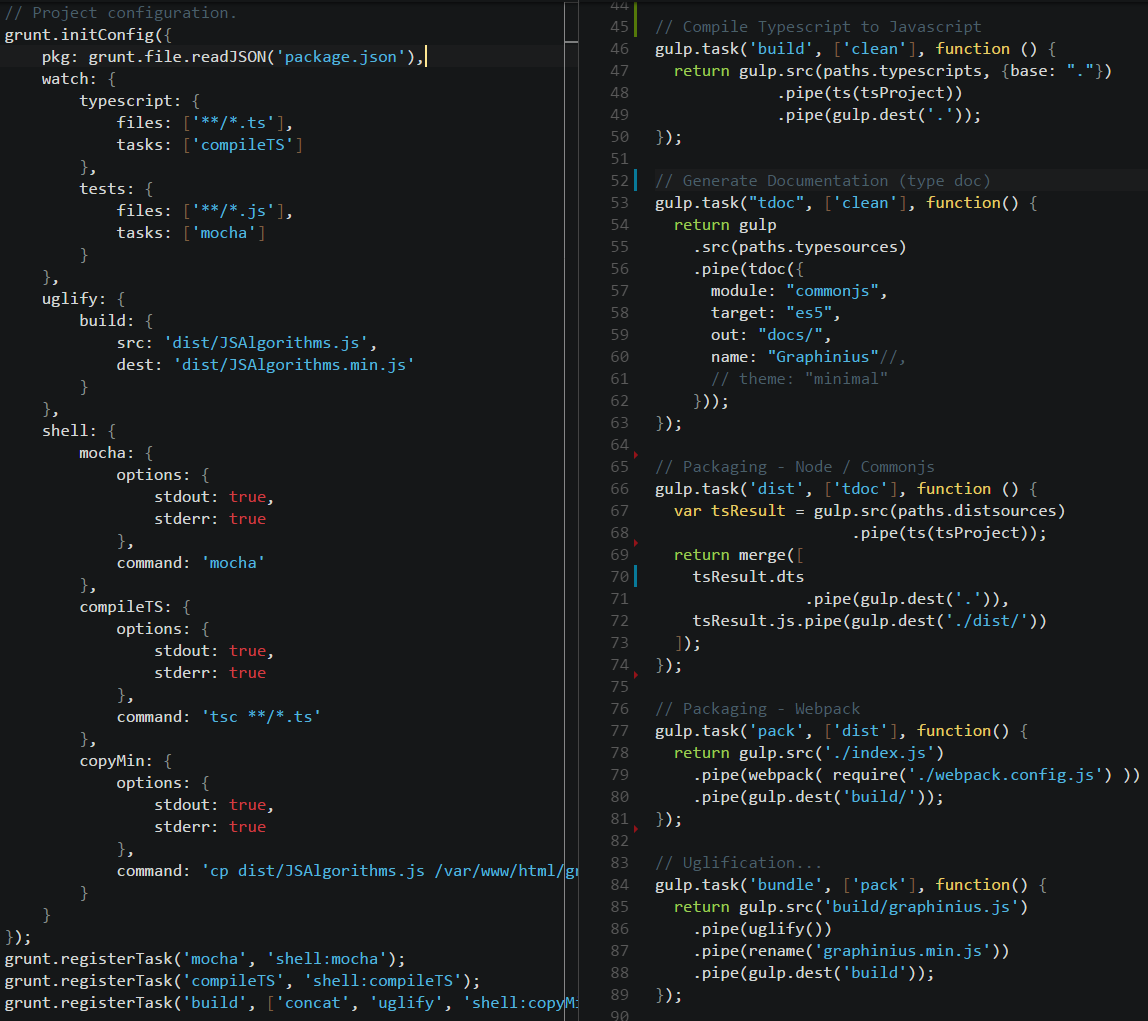
\includegraphics[width=1.2\textwidth]{figures/grunt_gulp_comparison}
			\caption{Comparison between Grunt \& Gulp build systems}
		\end{figure}
		
	






\section{Graphinius VIS}
\label{sect:graphinius_vis}

Description of Nicole's choices and decisions...

\begin{landscape}
\begin{figure}[ht]
	\label{fig_vis_control_flow}
	% \centering
	\hspace*{-1cm}
	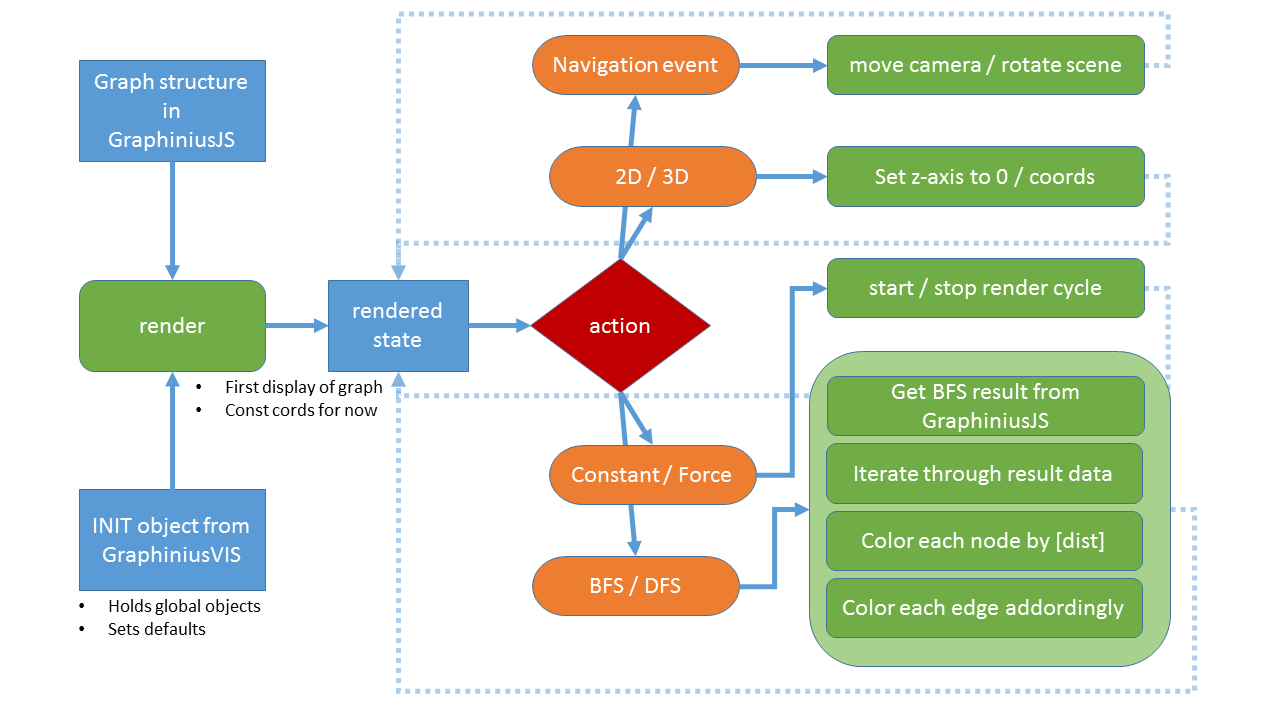
\includegraphics[width=1.9\textwidth]{figures/VIS_Control_Flow}
	\caption{Graphinius VIS control flow}
\end{figure}
\end{landscape}


